\documentclass[11pt]{beamer}
\usepackage[nosetup]{evan}
\usetheme{Malaysia}

\title{Welcome to 18.02 Recitation}
\subtitle{Mass Tech}
\author{Evan Chen}
\date{4 September 2024}

\begin{document}
\begin{frame}
  \maketitle
\end{frame}

\begin{frame}
  \frametitle{About me}
  \begin{itemize}
    \ii Evan Chen (\texttt{evan@evanchen.cc}), I'm a 5th-year grad student.
    \ii My recitation is MW 9am in 2-135 (right now).
    \ii My office hours is 10am in some room TBD.
    %\ii Warning: I've never taught a recitation before nor taken this class
  \end{itemize}
\end{frame}

\begin{frame}
  \begin{block}{Places to find things}
    \begin{itemize}
      \ii Canvas website has all the important course stuff
      \begin{itemize}
        \ii Piazza
        \ii Gradescope
      \end{itemize}
      \ii MIT-X has part of your problem sets
      \ii \url{https://web.evanchen.cc/1802.html} will have any
      optional supplemental stuff I make (like these slides), it's \alert{not} important
    \end{itemize}
  \end{block}
  \begin{block}{Dates}
    \begin{itemize}
      \ii Your first PSet is due Tue September 10. (It's shorter.)
      \ii Midterms are \alert{Fri Sept 27}, \alert{Tue Oct 22}, \alert{Fri Nov 15}.
      \begin{itemize}
        \ii Put these in your calendar right now, you do not want to miss them.
      \end{itemize}
      \ii Final TBD: don't book plane tickets home until date published.
    \end{itemize}
  \end{block}
\end{frame}

\begin{frame}
  \frametitle{What to expect}
  \begin{block}{Book}
    \begin{itemize}
      \ii First 7-ish lectures will actually be \alert{linear algebra} from Poonen's notes.
      No calculus at all!

      \ii Afterwards, switch to Edwards and Penney for actual calculus.
      \begin{itemize}
        \ii but tbh Poonen probably still better than E\&P.
      \end{itemize}
    \end{itemize}
  \end{block}
  \begin{block}{Class}
    \begin{itemize}
      \ii Lecture: Maulik teaches.
      \ii Recitation: Evan makes you do a worksheet.
      \begin{itemize}
        \ii (Today is unusual; future recitations won't have slides like this.)
        \ii Worksheets have about 4 problems but we won't cover them all.
        \ii Solutions posted later.
      \end{itemize}
      \ii Office hours: ask anything.
      \begin{itemize}
        \ii You can go to anyone's office hours.
      \end{itemize}
    \end{itemize}
  \end{block}
\end{frame}

\begin{frame}
  \frametitle{Advice you didn't ask for}
  \begin{center}
    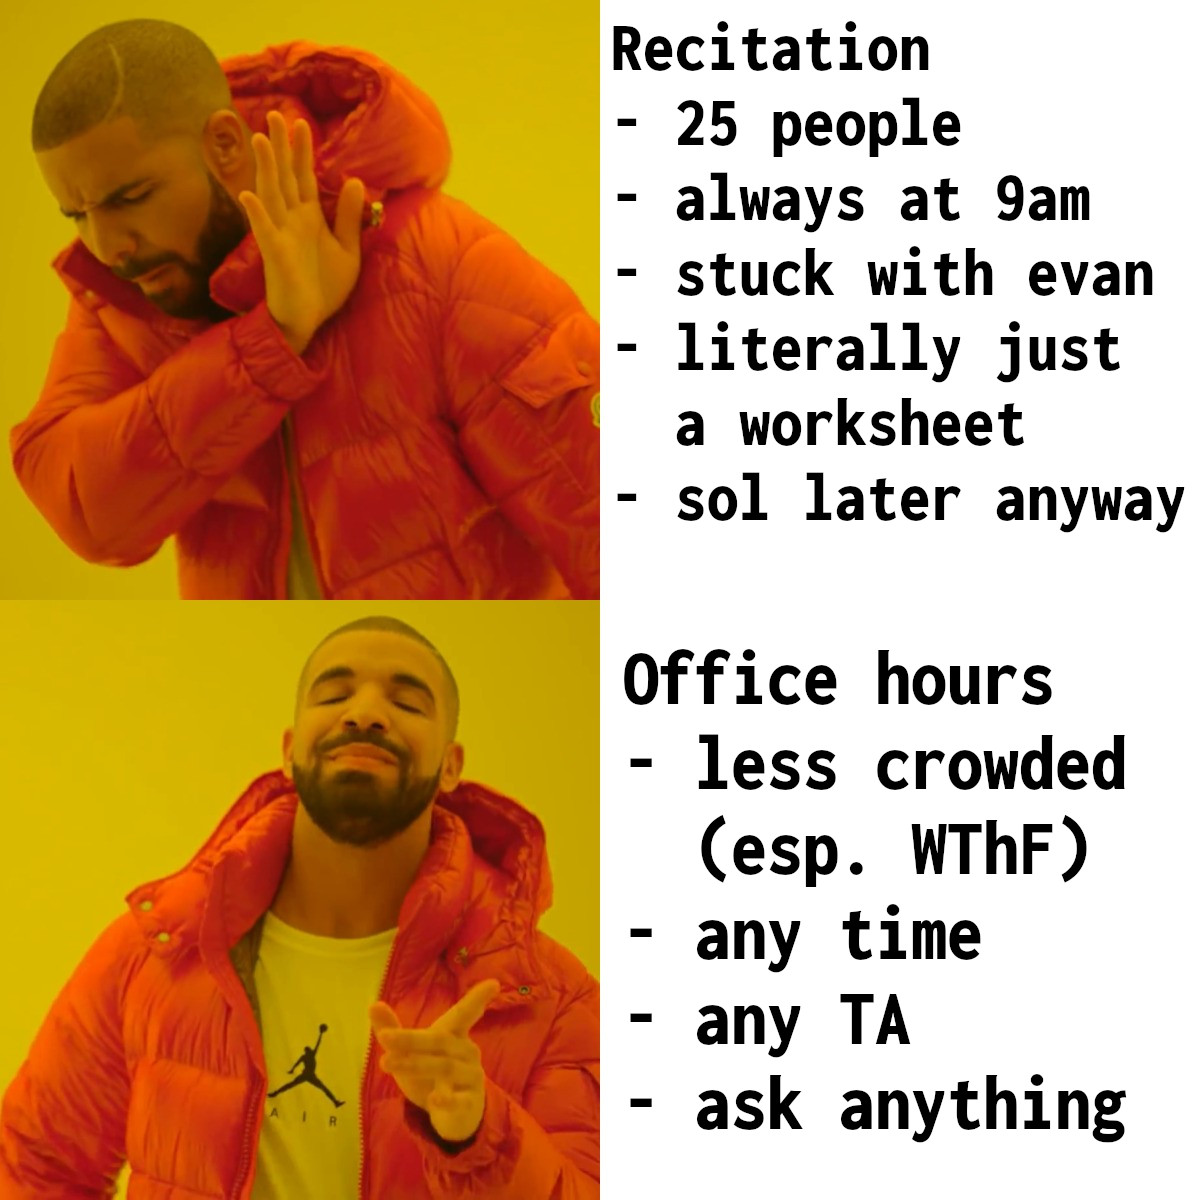
\includegraphics[width=0.6\textwidth]{hotline.jpg}
  \end{center}
\end{frame}

\begin{frame}
  \frametitle{Intro to vectors}
  \begin{alertblock}{Type safety (see printout)}
  Any time you see a new noun, verb, or adjective,
  make sure you know what \alert{types} of objects are involved.
  \end{alertblock}
  \begin{exampleblock}{Nouns you'll see this week}
    \begin{tabular}{llll}
      Term & Example & Notation & Container \\\hline
      Real num/scalar & $\frac23$, $\sqrt\pi$ & Lowercase ($r$, $\lambda$, \dots) & $\RR$ \\
      Vector & $\begin{bmatrix} 3 \\ 4 \end{bmatrix} = \left< 3,4 \right>$
             & $\vec v$, $\mathbf{v}$, $\overrightarrow{PQ}$, \dots & $\RR^n$ \\
             && $\mathbf{e}_1 = \mathbf{i} = \vec{\imath} = \left< 1,0,0 \right>$ \\
             && $\mathbf{e}_2 = \mathbf{j} = \vec{\jmath} = \left< 0,1,0 \right>$ \\
             && $\mathbf{e}_3 = \mathbf{k} = \vec{k} = \left< 0,0,1 \right>$ \\
      Matrix & $\begin{bmatrix} 1 & 2 \\ 3 & 4 \end{bmatrix}$ & Uppercase ($A$, $M$, \dots)
             & idk
    \end{tabular}
  \end{exampleblock}
\end{frame}

\begin{frame}
  \frametitle{Intro to vectors (cont'd)}
  \begin{block}{Fill in this table}
  \begin{tabular}{llllll}
    & & Notation & Type sig & Def (coords) & Pic \\ \hline
    \textbf{Vector} & noun \\
    \textbf{Len/mag} & verb \\
    \textbf{Unit} vector & adj \\
    \textbf{Scale} vector & verb \\
    \textbf{Add} vectors & verb \\
    \textbf{Subtract} vectors & verb \\
    \textbf{Dot prod.}\ (tmrw) & verb \\
  \end{tabular}
  \end{block}
\end{frame}


\end{document}
